\section{常数项级数的概念和性质}
人们认识事物在数量方面的特性,往往有一个由近似到精确的过程.
在这种认识过程中,会遇到由有限个数量相加到无穷多个数量相加的问题.

例如计算半径为\(R\)的圆面积\(A\),具体做法如下:
如\cref{figure:无穷级数.用内接正多边形覆盖圆},
作圆的内接正六边形,算出这六边形的面积\(a_1\),它是圆面积\(A\)的一个粗糙的近似值.
为了比较准确地计算出\(A\)的值,
我们以这个正六边形的每一边为底分别作一个顶点在圆周上的等腰三角形,
算出这六个等腰三角形的面积之和\(a_2\).
那么\(a_1+a_2\)(即内接正十二边形的面积)就是\(A\)的一个较好的近似值.
同样地,在这正十二边形的每一边上分别作一个顶点在圆周上的等腰三角形,
算出这十二个等腰三角形的面积之和\(a_3\).
那么\(a_1+a_2+a_3\)(即内接正二十四边形的面积)是\(A\)的一个更好的近似值.
如此继续下去,内接\(3\cdot2^n\)边形的面积就逐步逼近圆面积:\begin{equation*}
	A \approx a_1 + a_2 + \dotsb + a_n.
\end{equation*}

\begin{figure}[h]
%@see: 《高等数学(第六版 下册)》 P248 图12-1
	\centering
	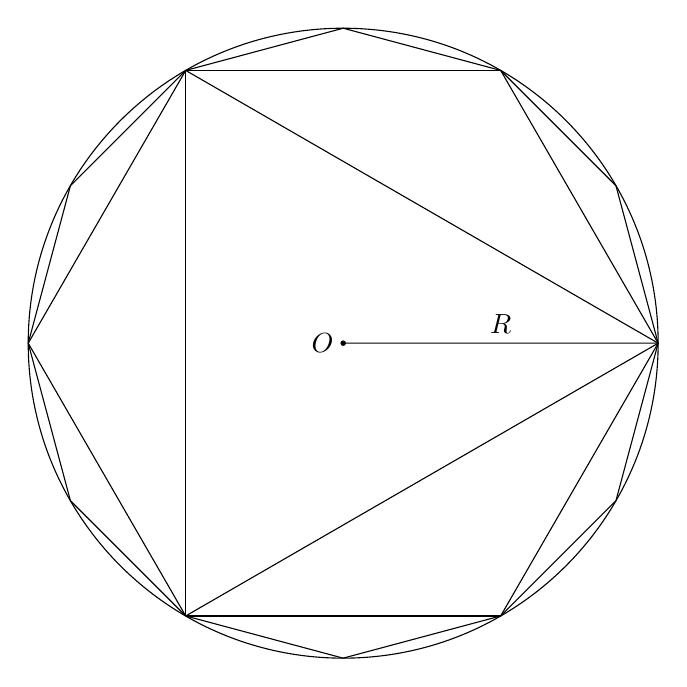
\begin{tikzpicture}
		\pgfmathsetmacro{\radius}{4}
		\def\PlotPolygon#1{
			\foreach \i in {1,...,#1}{
				\draw({\radius*cos(\i*360/#1)},{\radius*sin(\i*360/#1)})
				--({\radius*cos((\i-1)*360/#1)},{\radius*sin((\i-1)*360/#1)});
			}
		}
		\begin{scope}
			\PlotPolygon{3}
			\PlotPolygon{6}
			\PlotPolygon{12}
		\end{scope}
		\draw(0,0)circle(\radius)node[left]{\(O\)}
			--(\radius,0)node[midway,above]{\(R\)};
		\fill(0,0)circle(1pt);
	\end{tikzpicture}
	\caption{用内接正多边形覆盖圆}
	\label{figure:无穷级数.用内接正多边形覆盖圆}
\end{figure}

如果内接正多边形的边数无限增多,即\(n\)无限增大,
则和\(a_1+a_2+\dotsb+a_n\)的极限就是所要求的圆面积\(A\).
这时和式中的项数无限增多,于是出现了无穷多个数量依次相加的数学式子.

\subsection{常数项级数的概念}
\begin{definition}\label{definition:无穷级数.常数项级数的定义}
设\(\{u_n\}\)是数列.
定义:\begin{equation*}
	\sum_{n=1}^\infty u_n
	\defeq
	\lim_{n\to\infty} \sum_{k=1}^n u_k,
\end{equation*}
称之为\DefineConcept{常数项无穷级数}(infinite series with constant terms),
简称\DefineConcept{常数项级数},
或者进一步简称为\DefineConcept{级数}.
把\(u_n\)称为
“级数\(\sum_{n=1}^\infty u_n\)的\DefineConcept{一般项}”.
把\(\sum_{k=1}^n u_k\)称为
“级数\(\sum_{n=1}^\infty u_n\)的\DefineConcept{部分和}(partial sum)”.

如果级数\(\sum_{n=1}^\infty u_n\)的
部分和\(\sum_{k=1}^n u_k\)
构成的数列收敛于\(s\),
则称“级数\(\sum_{n=1}^\infty u_n\)~\DefineConcept{收敛}(converge)”,
我们把极限\(s\)叫做“级数\(\sum_{n=1}^\infty u_n\)的\DefineConcept{和}(sum)”.
反之,如果这个级数的部分和数列发散,
则称“级数\(\sum_{n=1}^\infty u_n\)~\DefineConcept{发散}(diverge)”.

当级数收敛时,
我们把收敛级数的和\(s\)与级数的部分和\(\sum_{k=1}^n u_k\)的差值\begin{equation*}
	\sum_{n=1}^\infty u_n - \sum_{k=1}^n u_k
\end{equation*}
叫做“级数\(\sum_{n=1}^\infty u_n\)的\DefineConcept{余项}”.
\end{definition}

\begin{example}\label{example:无穷级数.等比级数的收敛性}
%@see: 《数学分析(第二版 下册)》(陈纪修) P2 例9.1.1
级数\(\sum_{n=0}^\infty q^n\)
叫做\DefineConcept{等比级数}或\DefineConcept{几何级数}(geometric series).
%@see: https://mathworld.wolfram.com/GeometricSeries.html
我们把常数\(q\)叫做“级数\(\sum_{n=0}^\infty q^n\)的\DefineConcept{公比}”.
试讨论上述等比级数的收敛性.
\begin{solution}
根据\(q\)的取值范围,分情况讨论.
\begin{enumerate}
	\item 当\(q = 1\)时,则部分和为\begin{equation*}
		\sum_{i=0}^n q^n
		= n,
	\end{equation*}
	那么\(\lim_{n\to\infty} \sum_{i=0}^n q^n
	= \lim_{n\to\infty} n
	= \infty\),
	即级数发散.

	\item 当\(q \neq 1\),
	根据\cref{theorem:等比数列.前n项和} 有\begin{equation*}
		\sum_{i=0}^n q^n
		= \frac{1-q^n}{1-q}
		= \frac{1}{1-q} - \frac{q^n}{1-q}.
	\end{equation*}
	\begin{enumerate}
		\item 当\(\abs{q} < 1\)时,
		由于\(\lim_{n\to\infty} q^n=0\),
		从而\(\lim_{n\to\infty} \sum_{i=0}^n q^n
		=\frac{a}{1-q}\),
		因此级数收敛,
		其和为\(\frac{a}{1-q}\).

		\item 当\(\abs{q} > 1\)时,
		由于\(\lim_{n\to\infty} q^n=\infty\),
		从而\(\lim_{n\to\infty} \sum_{i=0}^n q^n
		=\infty\),
		级数发散.

		\item 当\(q = -1\)时,部分和为\begin{equation*}
			\sum_{i=0}^n q^n
			= \begin{cases}[cl]
				1, & \text{\(n\)是偶数}, \\
				0, & \text{\(n\)是奇数}.
			\end{cases}
		\end{equation*}
		根据\cref{theorem:子列极限.数列收敛的充分必要条件},
		\(\sum_{i=0}^n q^n\)的极限不存在,级数发散.
	\end{enumerate}
\end{enumerate}

综上所述,{\color{red}当\(\abs{q} < 1\)时,几何级数收敛;
当\(\abs{q} \geq 1\)时,几何级数发散.}
\end{solution}
\end{example}

\begin{example}\label{example:无穷级数.等差级数的收敛性}
试证:\DefineConcept{等差级数}(arithmetic series)\begin{equation*}
	1+2+3+\dotsb+n+\dotsb
\end{equation*}是发散的.
\begin{proof}
级数的部分和为\begin{equation*}
	s_n = 1+2+3+\dotsb+n = \frac{n(n+1)}{2}.
\end{equation*}
显然,\(\lim_{n\to\infty} s_n=\infty\),级数是发散的.
\end{proof}
%@see: https://mathworld.wolfram.com/ArithmeticSeries.html
\end{example}
从上例也可看出:
\begin{proposition}
除非初项\(a_0\)与公差\(d\)都等于\(0\),
否则等差级数\(\sum_{n=0}^\infty(a_0+nd)\)总是发散的.
\end{proposition}

\begin{example}
判定无穷级数\begin{equation*}
	\frac{1}{1\cdot2}+\frac{1}{2\cdot3}+\dotsb+\frac{1}{n(n+1)}+\dotsb
\end{equation*}的收敛性.
\begin{solution}
记\begin{equation*}
	u_n = \frac{1}{n(n+1)} = \frac{1}{n}-\frac{1}{n+1},
\end{equation*}
因此\begin{align*}
	s_n &= \frac{1}{1\cdot2}+\frac{1}{2\cdot3}+\dotsb+\frac{1}{n(n+1)} \\
	&= \left(1-\frac{1}{2}\right)+\left(\frac{1}{2}-\frac{1}{3}\right)
	+\dotsb+\left(\frac{1}{n}-\frac{1}{n+1}\right) \\
	&= 1-\frac{1}{n+1}.
\end{align*}
从而\begin{equation*}
	\lim_{n\to\infty} s_n
	= \lim_{n\to\infty} \left(1-\frac{1}{n+1}\right)
	= 1,
\end{equation*}
即该级数收敛,它的和为\(1\).
\end{solution}
\end{example}

\begin{example}\label{example:无穷级数.与调和数列有关的级数1}
%@see: https://www.bilibili.com/video/BV1c2yBYwEvt/
证明级数\(\sum_{n=1}^\infty \frac1{(n+1)(n+2)} \left( 1+\frac12+\dotsb+\frac1n \right)\)收敛并求和.
\begin{solution}
记\(a_n = 1+\frac12+\dotsb+\frac1n\),
那么\(a_n - a_{n-1} = \frac1n\ (n=2,3,\dotsc)\),
而级数的部分和为\begin{align*}
	S_n &= \sum_{k=1}^n \frac{a_k}{(k+1)(k+2)}
	% 裂项
	= \sum_{k=1}^n \left( \frac{a_k}{k+1} - \frac{a_k}{k+2} \right) \\
	&= \left( \frac{a_1}{2} - \frac{a_1}{3} \right)
	+ \left( \frac{a_2}{3} - \frac{a_2}{4} \right)
	+ \left( \frac{a_3}{4} - \frac{a_3}{5} \right)
	+ \dotsb + \left( \frac{a_{n-1}}{n} - \frac{a_{n-1}}{n+1} \right)
	+ \left( \frac{a_n}{n+1} - \frac{a_n}{n+2} \right) \\
	&= \frac{a_1}{2} + \frac{a_2 - a_1}{3}
	+ \frac{a_3 - a_4}{4} + \frac{a_4 - a_3}{5}
	+ \dotsb + \frac{a_n - a_{n-1}}{n+1}
	- \frac{a_n}{n+2} \\
	&= \frac1{2\cdot1} + \frac1{3\cdot2} + \frac1{4\cdot3} + \frac1{5\cdot4}
	+ \dotsb + \frac1{(n+1)n} - \frac{a_n}{n+2} \\
	% 裂项
	&= \left( 1-\frac12 \right) + \left( \frac12 - \frac13 \right)
	+ \dotsb + \left( \frac1n - \frac1{n+1} \right) - \frac{a_n}{n+2} \\
	&= 1 - \frac1{n+1} - \frac{a_n}{n+2}.
\end{align*}
这里\(\frac1{n+1}\to0\ (n\to\infty)\),
因此,要证部分和\(S_n\)收敛,需证数列\(\frac{a_n}{n+2}\)收敛.
由\cref{example:微分中值定理.拉格朗日中值定理.重要不等式1} 可知,
对于任意正整数\(n\)有\(\frac1{n+1} < \ln(1+\frac1n) < \frac1n\),
所以\begin{align*}
	a_n &= 1+\frac12+\frac13+\dotsb+\frac1n \\
	&< 1+\ln(1+\frac11)+\ln(1+\frac12)+\dotsb+\ln(1+\frac1{n-1}) \\
	&= 1+\ln2+\ln\frac32+\dotsb+\ln\frac{n}{n-1}
	= 1+\ln n,
\end{align*}
从而有\begin{equation*}
	0 < \frac{a_n}{n+2}
	< \frac{1+\ln n}{n+2}
	\to 0
	\quad(n\to\infty),
\end{equation*}
于是\(S_n\to1\ (n\to\infty)\),
即\(\sum_{n=1}^\infty \frac1{(n+1)(n+2)} \left( 1+\frac12+\dotsb+\frac1n \right) = 1\).
\end{solution}
\end{example}

\subsection{级数收敛的必要条件}
\begin{proposition}[级数收敛的必要条件]\label{theorem:无穷级数.级数收敛的必要条件}
%@see: 《高等数学(第六版 上册)》 P253 性质5(级数收敛的必要条件)
%@see: 《数学分析(第二版 上册)》(陈纪修) P3 定理9.1.1(级数收敛的必要条件)
如果级数\(\sum_{n=1}^\infty u_n\)收敛,
则它的一般项\(u_n\)收敛于\(0\),
即\begin{equation*}
	\lim_{n\to\infty} u_n = 0.
\end{equation*}
\begin{proof}
设级数\(\sum_{n=1}^\infty u_n\)的部分和为\(s_n\),
且\(\lim_{n\to\infty} s_n = s\),
则\begin{equation*}
	\lim_{n\to\infty} u_n
	= \lim_{n\to\infty}(s_n - s_{n-1})
	= \lim_{n\to\infty} s_n - \lim_{n\to\infty} s_{n-1}
	= s - s
	= 0.
	\qedhere
\end{equation*}
\end{proof}
\end{proposition}
\begin{remark}
数列\(\{u_n\}\)收敛\(\iff\)级数\(\sum_{n=1}^\infty (u_n - u_{n+1})\)收敛.
\end{remark}

值得注意的是,级数的一般项趋于零并不是级数收敛的充分条件.
有些级数虽然一般项趋于零,但仍然是发散的.
\begin{example}\label{example:无穷级数.调和级数的敛散性}
试证:\DefineConcept{调和级数}(harmonic series)\begin{equation*}
%@see: 《高等数学(第六版 上册)》 P253 (5)
	\sum_{n=1}^\infty u_n
	= 1+\frac12+\frac13+\dotsb+\frac1n+\dotsb
\end{equation*}是发散的.
\begin{proof}
虽然调和级数的一般项\(\lim_{n\to\infty} u_n
= \lim_{n\to\infty} 1/n
= 0\),
但是它是发散的.
现在我们用反证法证明.

假设级数\(\sum_{n=1}^\infty u_n\)收敛.
设级数的部分和为\(s_n\),
且\(\lim_{n\to\infty} s_n
= s\).
显然,对级数\(\sum_{n=1}^\infty u_n\)的部分和\(s_{2n}\)
也有\(\lim_{n\to\infty} s_{2n}
= s\).
于是\begin{equation*}
	\lim_{n\to\infty} (s_{2n}-s_n)
	= \lim_{n\to\infty} s_{2n} - \lim_{n\to\infty} s_n
	= s - s
	= 0.
\end{equation*}
但另一方面\begin{equation*}
	s_{2n} - s_n
	= \frac{1}{n+1}+\frac{1}{n+2}+\dotsb+\frac{1}{2n}
	> \underbrace{\frac{1}{2n}+\frac{1}{2n}+\dotsb+\frac{1}{2n}}_{\text{$n$项}}
	= n \cdot \frac1{2n}
	= \frac12,
\end{equation*}
由\cref{theorem:极限.收敛数列的保序性2} 可知\begin{equation*}
	\lim_{n\to\infty} (s_{2n}-s_n)
	\geq \frac12
	> 0,
\end{equation*}与假设矛盾,说明级数\(\sum_{n=1}^\infty u_n\)必定发散.
\end{proof}
%@see: https://mathworld.wolfram.com/HarmonicSeries.html
%@see: https://math.stackexchange.com/questions/1160527/the-series-sum-n-1-infty-frac1n-diverges
\end{example}

\begin{corollary}\label{theorem:无穷级数.级数收敛的必要条件.推论}
%@see: 《高等数学(第六版 上册)》 P253
%@see: https://mathworld.wolfram.com/DivergenceTests.html
%@see: https://mathworld.wolfram.com/LimitTest.html
如果级数\(\sum_{n=1}^\infty u_n\)的一般项不收敛于\(0\),
即\(u_n \not\to 0\ (n\to\infty)\),
那么\(\sum_{n=1}^\infty u_n\)发散.
\begin{proof}
\cref{theorem:无穷级数.级数收敛的必要条件} 的逆否命题.
\end{proof}
\end{corollary}

\begin{example}
%@see: 《高等数学(第六版 上册)》 P253
级数\begin{equation*}
	\frac12-\frac23+\frac34-\dotsb+(-1)^{n-1}\frac{n}{n+1}+\dotsb,
\end{equation*}的一般项
\(u_n = (-1)^{n-1} \frac{n}{n+1}\)满足\begin{equation*}
	\varlimsup_{n\to\infty} u_n = 1,
	\qquad
	\varliminf_{n\to\infty} u_n = -1,
\end{equation*}
于是\(u_n \not\to 0\ (n\to\infty)\),
由\cref{theorem:无穷级数.级数收敛的必要条件.推论} 可知,该级数是发散的.
\end{example}

即便在“级数的一般项趋于零”之外,再加上条件“级数的部分和数列有界”,也依然无法保证“级数收敛”.
\begin{example}
%@see: https://www.bilibili.com/video/BV1EkiGeJET3/
举例说明:当级数\(\sum_{n=1}^\infty a_n\)的部分和数列\(\{S_n\}\)有界
且\(\lim_{n\to\infty} a_n = 0\)时,
级数\(\sum_{n=1}^\infty a_n\)不收敛.
\begin{solution}
取\begin{equation*}
	a_n = \sin\sqrt{n+1} - \sin\sqrt{n}
	\quad(n=1,2,\dotsc),
\end{equation*}
那么由\hyperref[theorem:微分中值定理.拉格朗日中值定理]{拉格朗日中值定理}可知,
存在实数\(\xi\in(\sqrt{n},\sqrt{n+1})\),
使得\begin{equation*}
	\sin\sqrt{n+1} - \sin\sqrt{n}
	= \cos\xi \cdot (\sqrt{n+1} - \sqrt{n}).
\end{equation*}
由于\(\lim_{n\to\infty} (\sqrt{n+1} - \sqrt{n})
= \lim_{n\to\infty} \frac1{\sqrt{n+1} + \sqrt{n}}
= 0\),
而\(\cos\xi\)是有界量,
所以由\cref{theorem:函数极限.无穷小.有界函数与无穷小的乘积是无穷小}
可知\(\lim_{n\to\infty} a_n = 0\).
另一方面\begin{equation*}
	S_n = a_n + a_{n-1} + \dotsb + a_2 + a_1
	= \sin\sqrt{n+1} - \sin1
	\quad(n=1,2,\dotsc).
\end{equation*}
显然\(\{S_n\}\)有界但不收敛.
\end{solution}
\end{example}

\subsection{收敛级数的基本性质}
%@see: https://mathworld.wolfram.com/ConvergentSeries.html
\begin{property}\label{theorem:无穷级数.收敛级数性质1}
%@see: 《高等数学(第六版 上册)》 P251 性质1
%@see: 《数学分析(第二版 上册)》(陈纪修) P4 定理9.1.2(线性性)
如果级数\(\sum_{n=1}^\infty u_n\)收敛于和\(s\),
则级数\(\sum_{n=1}^\infty k u_n\)收敛于和\(ks\).
\begin{proof}
设级数\(\sum_{n=1}^\infty u_n\)
与级数\(\sum_{n=1}^\infty k u_n\)的
部分和分别为\(s_n\)与\(\sigma_n\),
则\begin{equation*}
	\sigma_n
	= k u_1 + k u_2 + \dotsb + k u_n
	= k(u_1 + u_2 + \dotsb + u_n) = k s_n,
\end{equation*}\begin{equation*}
	\lim_{n\to\infty} \sigma_n
	= \lim_{n\to\infty} k s_n
	= k \lim_{n\to\infty} s_n = ks,
\end{equation*}
也就是说,级数\(\sum_{n=1}^\infty k u_n\)收敛于\(ks\).
\end{proof}
\end{property}
\begin{remark}
由关系式\(\sigma_n = k s_n\)知道,
如果\(\{s_n\}\)没有极限且\(k\neq0\),
那么\(\{\sigma_n\}\)也不可能有极限.
因此我们得到如下结论:
{\color{red}级数的每一项同乘一个非零常数后,它的敛散性不会改变.}
\end{remark}
\begin{remark}
对于任意发散级数\(\sum_{n=1}^\infty u_n\),
级数\(\sum_{n=1}^\infty 0 \cdot u_n\)的每一项都是零,
故级数\(\sum_{n=1}^\infty 0 \cdot u_n\)收敛于\(0\).
\end{remark}

\begin{example}
判断\begin{equation*}
\sin\frac{\pi}{6}+\sin\frac{2\pi}{6}+\dotsb+\sin\frac{n\pi}{6}+\dotsb
\end{equation*}的收敛性.
\begin{solution}
记\(u_n = \sin\frac{n\pi}{6},
v_n = 2\sin\frac{\pi}{12} \cdot u_n\).
因为\begin{equation*}
	v_n = \cos\frac{\pi-2n\pi}{12} - \cos\frac{\pi+2n\pi}{12},
\end{equation*}\begin{equation*}
	\sigma_n
	= v_1 + v_2 + \dotsb + v_n
	= \cos\frac{\pi}{12} - \cos\frac{(2n+1)\pi}{12},
\end{equation*}
所以\begin{equation*}
	s_n
	= \left(2\sin\frac{\pi}{12}\right)^{-1} \cdot \sigma_n
	= 1+\frac{\sqrt{3}}{2} - \frac{\sqrt{2}}{\sqrt{3}-1} \cos\frac{(2n+1)\pi}{12}.
\end{equation*}
可见\(\lim_{n\to\infty} s_n\)不存在,级数发散.
\end{solution}
\end{example}

\begin{property}\label{theorem:无穷级数.收敛级数性质2}
%@see: 《高等数学(第六版 上册)》 P251 性质2
%@see: 《数学分析(第二版 上册)》(陈纪修) P4 定理9.1.2(线性性)
如果级数\(\sum_{n=1}^\infty u_n\)、\(\sum_{n=1}^\infty v_n\)
分别收敛于\(s\)、\(\sigma\),
则级数\(\sum_{n=1}^\infty(u_n \pm v_n)\)收敛于\(s \pm \sigma\).
\begin{proof}
设级数\(\sum_{n=1}^\infty u_n\)与级数\(\sum_{n=1}^\infty v_n\)的部分和
分别为\(s_n\)与\(\sigma_n\),
则级数\(\sum_{n=1}^\infty(u_n \pm v_n)\)的部分和\begin{align*}
	\tau_n &= (u_1 \pm v_1) + (u_2 \pm v_2) + \dotsb + (u_n + v_n) \\
	&= (u_1 + u_2 + \dotsb + u_n) \pm (v_1 + v_2 + \dotsb + v_n) \\
	&= s_n \pm \sigma_n,
\end{align*}
于是\begin{equation*}
	\lim_{n\to\infty} \tau_n
	= \lim_{n\to\infty} (s_n \pm \sigma_n)
	= s + \sigma.
\end{equation*}

这就表明级数\(\sum_{n=1}^\infty(u_n \pm v_n)\)收敛于\(s \pm \sigma\).
\end{proof}
\end{property}
\begin{remark}
从\cref{theorem:无穷级数.收敛级数性质1,theorem:无穷级数.收敛级数性质2} 可以看出:
对收敛级数可以进行加法和数乘运算.
\end{remark}

\begin{example}
设级数\(\sum_{n=1}^\infty u_n\)收敛,\(\sum_{n=1}^\infty v_n\)发散.
试证:级数\(\sum_{n=1}^\infty (u_n + v_n)\)发散.
\begin{proof}
设级数\(\sum_{n=1}^\infty u_n\)与\(\sum_{n=1}^\infty v_n\)的部分和
分别为\(s_n\)和\(\sigma_n\),
又设\begin{equation*}
	\lim_{n\to\infty} s_n = s.
\end{equation*}
用反证法.
假设级数\(\sum_{n=1}^\infty (u_n + v_n)\)收敛于\(s + \sigma\),
即\begin{equation*}
	\lim_{n\to\infty} (s_n + \sigma_n) = s+\sigma,
\end{equation*}
那么根据\hyperref[theorem:极限.极限的四则运算法则]{极限的四则运算法则},
有\begin{equation*}
	\lim_{n\to\infty} \sigma_n
	= \lim_{n\to\infty} [(s_n + \sigma_n) - s_n]
	= \lim_{n\to\infty} (s_n + \sigma_n) - \lim_{n\to\infty} s_n
	= (s + \sigma) - s
	= \sigma,
\end{equation*}
也就是说级数\(\sum_{n=1}^\infty v_n\)的部分和数列\(\{\sigma_n\}\)收敛,
于是级数\(\sum_{n=1}^\infty v_n\)收敛,矛盾!
因此级数\(\sum_{n=1}^\infty (u_n + v_n)\)必定发散.
\end{proof}
\end{example}

从上例我们可以看出:
\begin{proposition}\label{theorem:无穷级数.收敛级数性质2.推论1}
一个收敛级数与一个发散级数相加(或相减)所得级数必定发散.
\end{proposition}

另一方面,任给一个发散级数\(\sum_{n=1}^\infty u_n\),
级数\(\sum_{n=1}^\infty u_n + \sum_{n=1}^\infty u_n
= \sum_{n=1}^\infty 2 u_n\)也是发散的,
而级数\(\sum_{n=1}^\infty u_n - \sum_{n=1}^\infty u_n
= 0\)却是收敛的,
于是我们还可以看出:
{\color{red}两个发散级数相加(或相减)所得级数可能收敛也可能发散.}

\begin{example}
已知级数\(\sum_{n=1}^\infty (-1)^{n-1} a_n = 2,
\sum_{n=1}^\infty a_{2n-1} = 5\),
求\(\sum_{n=1}^\infty a_n\).
\begin{solution}
由于\(\sum_{n=1}^\infty [a_n + (-1)^{n-1} a_n]
= 2 \sum_{n=1}^\infty a_{2n-1}\)收敛,
所以\(\sum_{n=1}^\infty a_n\)收敛,且有
\begin{equation*}
\sum_{n=1}^\infty a_n
= 2 \sum_{n=1}^\infty a_{2n-1}
- \sum_{n=1}^\infty (-1)^{n-1} a_n
= 10 - 2 = 8.
\end{equation*}
\end{solution}
\end{example}

\begin{property}\label{theorem:无穷级数.收敛级数性质3}
%@see: 《高等数学(第六版 上册)》 P252 性质3
在级数中去掉、加上或改变有限项,不会改变级数的收敛性.
\begin{proof}
我们只需证明“在级数的前面部分去掉或加上有限项,不会改变级数的收敛性”,
因为其他情形(即在级数中任意去掉、加上或改变有限项的情形)都可以看成在级数的前面部分先去掉有限项,
然后再加上有限项的结果.

将级数\begin{equation*}
u_1+u_2+\dotsb+u_k+u_{k+1}+\dotsb+u_{k+n}+\dotsb
\end{equation*}的前\(k\)项去掉,则得级数\begin{equation*}
u_{k+1}+u_{k+2}+\dotsb+u_{k+n}+\dotsb.
\end{equation*}于是新得到的级数的部分和为\begin{equation*}
\sigma_n = u_{k+1}+u_{k+2}+\dotsb+u_{k+n} = s_{k+n} - s_k,
\end{equation*}其中\(s_{k+n}\)是原级数的前\(k+n\)项的和.
因为\(s_k\)是常数,所以当\(n\to\infty\)时,
\(\sigma_n\)与\(s_{k+n}\)这两个量,要么同时具有极限,要么同时没有极限.

同理可证在级数的前面加上有限项,不会改变级数的收敛性.
由此可见,在级数中去掉、加上或改变有限项,不会改变级数的收敛性.

另外,我们可以观察到,在收敛级数中去掉、加上或改变有限项,
虽不会改变级数的收敛性,但可能会改变收敛级数的和.
\end{proof}
\end{property}

\begin{property}\label{theorem:无穷级数.收敛级数性质4}
%@see: 《高等数学(第六版 上册)》 P252 性质4
%@see: 《数学分析(第二版 上册)》(陈纪修) P4 定理9.1.3
如果级数\(\sum_{n=1}^\infty u_n\)收敛,
则对这级数的项任意加括号后所成的级数\begin{equation*}
%@see: 《高等数学(第六版 上册)》 P252 (4)
	(u_1+\dotsb+u_{n_1})
	+ (u_{n_1+1}+\dotsb+u_{n_2})
	+ \dotsb
	+ (u_{n_{k-1}+1}+\dotsb+u_{n_k}) + \dotsb
\end{equation*}仍收敛,且其和不变.
\begin{proof}
设\(\sum_{n=1}^\infty u_n\)添加括号后表示为\begin{align*}
	&(u_1 + u_2 + \dotsb + u_{n_1}) \\
	&+ (u_{n_1+1} + u_{n_1+2} + \dotsb + u_{n_2}) \\
	&+ \dotsb + (u_{n_{k-1}+1} + u_{n_{k-1}+2} + \dotsb + u_{n_k}) + \dotsb.
\end{align*}
令\begin{equation*}
	\begin{array}{l}
		v_1 = u_1 + u_2 + \dotsb + u_{n_1}, \\
		v_2 = u_{n_1+1} + u_{n_1+2} + \dotsb + u_{n_2}, \\
		\hdotsfor{1} \\
		v_k = u_{n_{k-1}+1} + u_{n_{k-1}+2} + \dotsb + u_{n_k}, \\
		\hdotsfor{1}
	\end{array}
\end{equation*}
则\(\sum_{n=1}^\infty u_n\)按上面上述方式添加括号后所得的级数为\(\sum_{n=1}^\infty v_n\).

设\(\sum_{n=1}^\infty u_n\)的部分和数列为\(\{S_n\}\),
\(\sum_{n=1}^\infty v_n\)的部分和数列为\(\{S'_n\}\),
则\begin{equation*}
	S'_1 = S_{n_1},
	S'_2 = S_{n_2},
	\dotsc,
	S'_k = S_{n_k},
	\dotsc
\end{equation*}
显然\(\{S'_n\}\)是\(\{S_n\}\)的一个子列,
于是由\(\{S_n\}\)的收敛性可得\(\{S'_n\}\)的收敛性,
且两者极限相同.
\end{proof}
\end{property}
\begin{remark}
\cref{theorem:无穷级数.收敛级数性质4} 说明:
收敛的级数满足加法结合律.
\end{remark}
\begin{remark}
在极限论中我们已经知道,一个数列的某个子列收敛并不能保证数列本身收敛.
因此,相应地,在一个级数的和式中,添加了括号后所得的级数收敛,并不能保证原来的级数收敛.
例如,级数\begin{equation*}
	1-1+1-1+\dotsb
\end{equation*}是发散的,
但是,加上括号以后,级数\begin{equation*}
	(1-1)+(1-1)+\dotsb
\end{equation*}收敛于\(0\),
而级数\begin{equation*}
	1+(-1+1)+(-1+1)+\dotsb
\end{equation*}收敛于\(1\).
这就说明,发散的级数不满足加法结合律.
\end{remark}
\begin{corollary}
如果加括号后所成的级数发散,则原来的级数也发散.
\begin{proof}
用反证法.
倘若原级数收敛,
则根据\cref{theorem:无穷级数.收敛级数性质4} 知道,
加括号后的级数就应该收敛了.
\end{proof}
\end{corollary}

\subsection{柯西审敛原理}
由于无穷级数\(\sum_{n=1}^\infty u_n\)收敛
即为极限\(\lim_{n\to\infty} \sum_{k=1}^n u_k\)存在,
对无穷级数收敛性的最本质的刻画,
就是极限论中的\hyperref[theorem:极限.函数的柯西极限存在准则]{柯西极限存在准则},
它可以表述为如下形式:
\begin{theorem}[柯西审敛原理]\label{theorem:无穷级数.级数的柯西审敛原理}
%@see: 《高等数学(第六版 下册)》 P254 柯西审敛原理
%@see: 《数学分析(第二版 下册)》(陈纪修) P29 定理9.4.1(级数的Cauchy收敛原理)
%@see: 《数学分析教程(第3版 下册)》(史济怀) P180 定理14.4.1(Cauchy收敛原理)
%@see: 《数学分析(第2册)》(周民强) P170 定理9.14
级数\(\sum_{n=1}^\infty u_n\)收敛的充分必要条件为:
对于任意给定的正数\(\epsilon\),
总存在正整数\(N\),
使得当\(n>N\)时,
对于任意的正整数\(m\),
总是成立\begin{equation*}
	\abs{ \sum_{k=1}^m u_{n+k} }
	< \epsilon.
\end{equation*}
\end{theorem}

我们可以利用极限记号,
把\hyperref[theorem:无穷级数.级数的柯西审敛原理]{柯西审敛原理}改写为如下命题.
\begin{proposition}
级数\(\sum_{n=1}^\infty u_n\)收敛的充分必要条件是:
对于任意正整数\(m\),总有\begin{equation*}
	\lim_{n\to\infty} \sum_{k=1}^m u_{n+k} = 0.
\end{equation*}
\end{proposition}

\begin{example}\label{example:无穷级数.zeta2的敛散性}
试求级数\(\sum_{n=1}^\infty \frac{1}{n^2}\)的收敛性.
\begin{solution}
因为对任意正整数\(p\),\begin{align*}
	&\abs{u_{n+1}+u_{n+2}+\dotsb+u_{n+p}} \\
	&=\frac{1}{(n+1)^2}+\frac{1}{(n+2)^2}+\dotsb+\frac{1}{(n+p)^2} \\
	&<\frac{1}{n(n+1)}+\frac{1}{(n+1)(n+2)}+\dotsb+\frac{1}{(n+p-1)(n+p)} \\
	&=\left(\frac{1}{n}-\frac{1}{n+1}\right)
		+\left(\frac{1}{n+1}-\frac{1}{n+2}\right)
		+\dotsb+\left(\frac{1}{n+p-1}-\frac{1}{n+p}\right) \\
	&=\frac{1}{n}-\frac{1}{n+p} < \frac{1}{n},
\end{align*}
所以对于\(\forall \epsilon > 0\),
取正整数\(N \geq \frac{1}{\epsilon}\),
则当\(n > N\)时,
对任何正整数\(p\),
都有\begin{equation*}
	\abs{u_{n+1}+u_{n+2}+\dotsb+u_{n+p}}
	< \frac{1}{n}
	< \frac{1}{N}
	\leq \epsilon
\end{equation*}成立.
按柯西审敛原理,级数\(\sum_{n=1}^\infty \frac{1}{n^2}\)收敛.
\end{solution}
\end{example}

\begin{example}
%@see: 《数学分析(第2册)》(周民强) P171 例1
设\(\{u_n\}\)是单调增加的无界的正数列.
证明:级数\(\sum_{n=1}^\infty \left(1-\frac{u_n}{u_{n+1}}\right)\)发散.
\begin{proof}
显然\(u_n\to+\infty\ (n\to\infty)\),
那么对于任意给定正整数\(N\),
当\(p\)充分大时,
有\begin{equation*}
	u_{N+p} > 2 u_N.
\end{equation*}
从而有\begin{align*}
	&\sum_{n=N}^{N+p} \left(1-\frac{u_n}{u_{n+1}}\right)
	= \sum_{n=N}^{N+p} u_n \left(\frac1{u_n}-\frac1{u_{n+1}}\right) \\
	&\geq u_N \left(\frac1{u_N}-\frac1{u_{N+p+1}}\right)
	= 1-\frac{u_N}{u_{N+p+1}}
	> \frac12.
\end{align*}
于是由{柯西审敛原理}可知级数\(\sum_{n=1}^\infty \left(1-\frac{u_n}{u_{n+1}}\right)\)发散.
\end{proof}
\end{example}

\begin{example}
%@see: 《数学分析(第2册)》(周民强) P171 例2
设\(a_n>0\ (n=1,2,\dotsc)\),\(p>0\),
级数\(\sum_{n=1}^\infty \frac{a_n}{n^p}\)收敛.
证明:\(\lim_{n\to\infty} \sum_{k=1}^n \frac{a_k}{n^p} = 0\).
\begin{proof}
因为级数\(\sum_{n=1}^\infty \frac{a_n}{n^p}\)收敛,
由{柯西审敛原理}可知,
对任意给定\(\epsilon>0\),
存在正整数\(N_1\),
对于任意正整数\(n \geq N_1\),
成立\begin{equation*}
	% N_1 \leq k \leq n
	% \implies
	% 0 < \frac1n \leq \frac1k
	% \implies
	\sum_{k=N_1+1}^n \frac{a_k}{n^p}
	< \sum_{k=N_1+1}^n \frac{a_k}{k^p}
	< \epsilon,
\end{equation*}
又因为\(\lim_{n\to\infty} \sum_{k=1}^{N_1} \frac{a_k}{n^p} = 0\),
故同时存在正整数\(N_2\),
当\(n > N_2\)时,
成立\begin{equation*}
	\sum_{k=1}^{N_1} \frac{a_k}{n^p}
	\leq \frac{N_1}{n^p} \cdot \max_{1 \leq k \leq N_1} a_k
	< \epsilon,
\end{equation*}
于是,当\(n>\max\{N_1,N_2\}\)时,成立\begin{equation*}
	\sum_{k=1}^n \frac{a_k}{n^p}
	= \sum_{k=N_1+1}^n \frac{a_k}{n^p}
	+ \sum_{k=1}^{N_1} \frac{a_k}{n^p}
	< 2\epsilon,
\end{equation*}
这就说明\(\lim_{n\to\infty} \sum_{k=1}^n \frac{a_k}{n^p} = 0\).
\end{proof}
\end{example}

\begin{example}
%@see: 《数学分析(第二版 下册)》(陈纪修) P43 习题 3.
%@see: 《数学分析(第2册)》(周民强) P150 定理9.6(Pringsheim)
设正项级数\(\sum_{n=1}^\infty u_n\)收敛,数列\(\{u_n\}\)单调减少.
利用柯西审敛原理证明:\(\lim_{n\to\infty} n u_n = 0\).
\begin{proof}
由于级数\(\sum_{n=1}^\infty u_n\)收敛,数列\(\{u_n\}\)单调减少,
所以对于任意给定\(\epsilon>0\),
存在正整数\(N\),使得当\(n>N\)时,
对于任意正整数\(m\),总是成立\begin{equation*}
	m \cdot u_{n+m}
	< \abs{\sum_{k=1}^m u_{n+k}}
	= u_{n+1} + u_{n+2} + \dotsb + u_{n+m}
	< \epsilon.
\end{equation*}

令\(m=n\),
则\(n u_{2n} < \epsilon\),
于是\(\lim_{n\to\infty} n u_{2n} = 0\).

又令\(m=n-1\),
则\((n-1) u_{2n-1} < \epsilon\),
于是\(\lim_{n\to\infty} (n-1) u_{2n-1} = 0\).

考虑到\(\lim_{n\to\infty} u_n = 0\),
于是又有\(\lim_{n\to\infty} (2n-1) u_{2n-1} = 0\).

综上所述,\(\lim_{n\to\infty} n u_n = 0\).
\end{proof}
\end{example}
